\chapter{Feature representation variability}\label{chap:feature-variation}
When translating input SVGs into feature vectors, we have to make key decisions about how SVG commands are specifically transformed into the nine-dimensional encoding that our model accepts as input.
Some examples of variation are:

\begin{itemize}
\item \textbf{Absolute vs.\ relative coordinates}: are start, end, and control points represented in terms of their absolute position in the drawing or their relative displacement between each other?
\item \textbf{Coordinate system orientation}: if relative, do we specify displacement vectors in terms of the normal $\{(1, 0), (0, 1)\}$ basis, or do we transform their values such that they represent deviations from continuing in the same direction as the previous point?
\item \textbf{Pairwise coordinate choice}: if relative, between which points in the curves' coordinate parameters do we measure displacement?
\end{itemize}

Here, we report results of an experiment in which we find that alternative forms of our feature adaptation process have varying ``learnability''; training differently transformed inputs with the same model architecture produces outputs of varying quality.

\section{Evaluating feature encodings}\label{sec:eval-encs}
To investigate the effects of choices for the above questions, we train five models each with a different feature encoding for input and output drawings.
Code for generating each encoding can be found in Appendix~\ref{app:enc}.

\begin{table}[t]
\centering
\caption[Feature encoding variants]{The differences between the five feature representations used for the encoding efficacy experiment.
    Each feature encoding uses six dimensions for the cubic B\'ezier parameters (two for each point vector) and three for the pen state (pen up, pen down, end drawing).
    Note that \code{s} represents the start coordinates of the curve, \code{e} represents the end coordinates of the curve, \code{c1} represents the coordinates of the curve's first control point, and \code{c2} represents the coordinates of the curve's second control point.
    \code{disp(a, b)} indicates displacement between points \code{a} and \code{b}, and \code{rot(v)} indicates that vector \code{v} has been rotated such that its coordinates are in the direction of the previous vector in the encoding.\label{tbl:features}}
\begin{tabularx}{\linewidth}{c X}
\toprule
    Encoding & Feature vector description \\ \midrule
    A & \code{disp(s, e), disp(s, c1), disp(s, c2), pen\_state}\\
    B & \code{disp(s, c1), disp(c1, c2), disp(c2, e), pen\_state}\\
    C & \code{disp(s, e), rot(disp(s, c1)), rot(disp(c2, e)), pen\_state}\\
    D & \code{e, rot(disp(s, c1)), rot(disp(c2, e)), pen\_state}\\
    E & \code{e, c1, c2, pen\_state}\\
\end{tabularx}
\end{table}

All models are trained using the same architecture as described in Chapter~\ref{chap:architecture} for 125k steps.
To generate the differently encoded inputs, the same base dataset of SVGs for the glyph \textbf{b} in various font faces is transformed to produce a list of feature vectors per glyph for each representation in Table~\ref{tbl:features}.
The base dataset is then partitioned randomly into 1920 training examples, 240 validation examples, and 240 test examples.
We follow the original training procedure described in Section~\ref{sec:training} with the same hyperparameters.
Training loss graphs and test loss values are included in Appendix~\ref{app:train}.

\section{Results}
We evaluate results quantitatively by computing the Hausdorff similarity metric between each ground truth image and a corresponding image conditionally generated by the model with $\tau = 0.3$, using the same method as described in Section~\ref{sec:quant-eval}.
Evaluation is run on a set of $N$ test set images for each encoding, and quantitative results are reported in Table~\ref{tbl:encoding-results}.
Sample conditionally generated images can be found in Figure~\ref{fig:encodings}.

\begin{table}[t]
\centering
\caption[Quantitative results for evaluating feature encodings]
    {Modified Hausdorff distance between conditionally generated and ground truth images for models trained on the \textbf{b} dataset with each encoding on a test set of $N$ images.
    Some pairs are omitted from comparison because the model failed to decode inputs into a valid (non-null) output.\label{tbl:encoding-results}}
\begin{tabular}{c c c c c}
\toprule
    Encoding & Mean & Std.\ dev. & Kurtosis & $N$ pairs \\ \midrule
    A & 28.7707 & 11.9332 & 1.3354 & 239 \\
    B & 15.4189 & 8.4912 & 3.1740 & 239 \\
    C & 24.8122 & 14.5086 & 17.9476 & 233 \\
    D & 15.9723 & 7.6134 & 0.9394 & 240 \\
    E & 16.7207 & 7.1926 & 0.8920 & 240 \\
\end{tabular}
\end{table}

While encoding E maintains high image similarity as measured by the Hausdorff metric, its generated outputs tend to lack smooth curves and straight lines and are characterized instead by jagged, bite-mark shaped curves.
This demonstrates a potential shortcoming of our Hausdorff similarity metric: training a model on strokes' absolute positions seems to result in greater preservation of the original glyph shape but may make learning style properties more difficult.

Encodings B and D seem to result in the glyphs most visually similar to ground truth glyphs and score relatively well on generated image similarity.
We interpret this finding as suggesting that the model learns style and structure better when SVG data is encoded such that features represent displacement between adjacent control points---for example, start point and first control point, or second control point and end point.
Based on this experiment, we use encoding B for our model evaluations in Chapters~\ref{chap:training} and~\ref{chap:style}.

\begin{figure}[t]
    \centering
	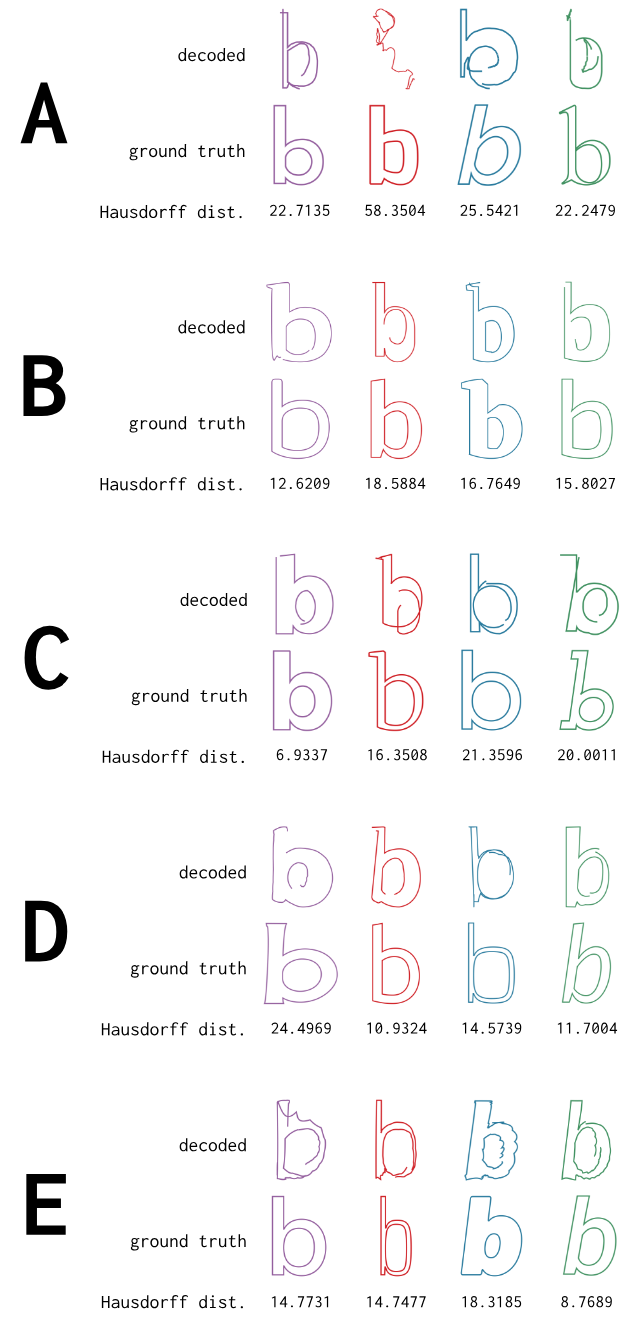
\includegraphics[height=0.8\textheight]{figures/encodings}
    \caption[Visual results of training the SVG model with different encodings]
    {Randomly sampled input-output pairs from the SVG models trained on the five encodings described in Table~\ref{tbl:features}.
    Decoded outputs were generated at $\tau = 0.3$.
    Decoded outputs are found in the top row for each encoding, while ground truth inputs are in the bottom row.\label{fig:encodings}}
\end{figure}

